\documentclass[margin=0px]{article}

\usepackage{listings}
\usepackage[utf8]{inputenc}
\usepackage{graphicx}
\usepackage{float}
\usepackage[a4paper, margin=0.7in]{geometry}
\usepackage{amsthm}
\usepackage{amssymb}
\usepackage{fancyhdr}
\usepackage{setspace}

\onehalfspacing

\renewcommand{\figurename}{ábra}

\newenvironment{tetel}[1]{\paragraph{#1}}{}

\pagestyle{fancy}
\lhead{\it{PTI BSc Záróvizsga tételek}}
\rhead{19. Osztott rendszerek és konkurens programozás}

\title{\textbf{{\Large ELTE IK - Programtervező Informatikus BSc} \vspace{0.2cm} \\ {\huge Záróvizsga tételek}} \vspace{0.3cm} \\ 19. Osztott rendszerek és konkurens programozás}
\author{}
\date{}

\begin{document}
\maketitle

\begin{tetel}{Osztott rendszerek és konkurens programozás}
    \begin{itemize}
        \item[] \textbf{A, C}: Folyamat fogalma, elosztott rendszerek tulajdonságai és felépítése, elnevezési rendszerek, kommunikáció, szinkronizáció, konzisztencia.
        \item[] \textbf{B}: Feladatok specifikációja biztonsági és haladási feltételekkel, absztrakt párhuzamos program tulajdonságai, megoldás fogalma, nevezetes feladatok megoldása párhuzamos és elosztott programokkal.
        \item[] \textbf{2018}: Szálkezelés. Ütemezés, kontextusváltás. Race condition. Szinkronizáció. Blokkoló műveletek. Memória (stack és heap) használata a szálakban. A konkurens programozás nyelvi eszközei. Szinkronizációhoz és kommunikációhoz használható adatszerkezetek.
    \end{itemize}
\end{tetel}

\section{Folyamatok, szálak}

\noindent \textbf{Szál}: A szál (thread) a processzor egyfajta szoftveres megfelelője, minimális kontextussal. Ha a szálat
megállítjuk, a kontextus elmenthető és továbbfuttatáshoz visszatölthető.\\

\noindent \textbf{Folyamat}: A folyamat (process vagy task) egy vagy több szálat összefogó nagyobb egység. Egy folyamat
szálai közös memóriaterületen (címtartományon) dolgoznak, azonban különböző folyamatok nem látják egymás memóriaterületét.\\

\noindent \textbf{Kontextusváltás}: A másik folyamatnak/szálnak történő vezérlésátadás, így egy processzor több szálat/ folyamatot
is végre tud hajtani.\\

\noindent \textbf{Szál vs. folyamat}: A szálak közötti váltáshoz nem kell igénybe venni az oprendszer szolgáltatásait, míg
a folyamatok közötti váltásnál ahhoz, hogy a régi és új folyamat memóriaterülete elkülönüljön a memóriavezérlő (MMU)
tartalmának jó részét át kell írni, amihez csak a kernel szintnek van joga. A folyamatok létrehozása, törlése és a kontextusváltás
közöttük sokkal költségesebb a szálakénál.

\section{Elosztott rendszerek tulajdonságai és felépítése}

\noindent \textbf{Elosztott rendszer fogalma}: Az elosztott rendszer önálló számítógépek olyan összessége, amely kezelői számára
egyetlen koherens rendszernek tűnik.

\subsection{Az elosztott rendszer céljai, tulajdonságai}

Az elosztott rendszer céljai a következők:

\begin{itemize}
    \item	Távoli erőforrások elérhetővé tétele

    \item	Átlátszóság (transparency)

    \item	Nyitottság (openness)

    \item	Skálázhatóság
\end{itemize}

\subsubsection{Átlátszóság}

Az átlátszóság nem más, mint az erőforrásokkal kapcsolatos különböző információk elrejtése a felhasználó elől.
Az alapján, hogy mit rejtünk el, többféle fajtája létezik:

\begin{figure}[H]
    \centering
    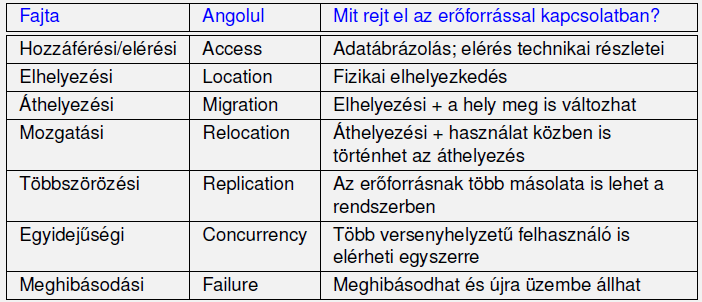
\includegraphics[width=0.8\linewidth]{img/atlatszosag}
    \caption{Az átlátszóság különböző típusai.}
    \label{fig:atlatszosag}
\end{figure}

\subsubsection{Nyitottság}

A rendszer képes más nyitott rendszerek számára szolgáltatásokat nyújtani, és azok szolgáltatásait igénybe venni:

\begin{itemize}
    \item	A rendszerek jól definiált interfészekkel rendelkeznek.
    \item	Az alkalmazások hordozhatóságát (portability) minél inkább támogatják.
    \item	Könnyen elérhető a rendszerek együttműködése.
\end{itemize}

\noindent A nyitott elosztott rendszer legyen könnyen alkalmazható heterogén környezetben, azaz
különböző hardvereken, platformokon, programozási nyelveken.\\

\noindent \textbf{Implementálása}:

\begin{itemize}
    \item	Fontos, hogy a rendszer könnyen cserélhető elemekből álljon.
    \item	Belső interfészek használata, nem egyetlen monolitikus rendszer.
    \item	A rendszernek minél jobban paraméterezhetőnek kell lennie.
    \item	Egyetlen komponens megváltoztatása/cseréje lehetőleg minél kevésbé
          hasson a rendszer más részeire.
\end{itemize}

\subsubsection{Skálázhatóság}

Többféle jelentése van, 3 fontos dimenzió:

\begin{enumerate}
    \item	méret szerinti skálázhatóság: a felhasználók és/vagy folyamatok száma
    \item	földrajzi skálázhatóság: a csúcsok közötti legnagyobb távolság
    \item	adminisztrációs skálázhatóság: az adminisztrációs tartományok száma
\end{enumerate}

Ezek közül a legtöbb rendszer a méret szerinti skálázhatóságot kezeli, ennek egy lehetséges megvalósítási
módja erősebb szerverek használata. A másik kettőt nehezebb kezelni.\\

\noindent Technikák a skálázhatóság megvalósítására:

\begin{itemize}
    \item	A kommunikációs késleltetés elfedése azzal, hogy a válaszra várás közben más tevékenységet végzünk. Ehhez
          aszinkron kommunikáció szükséges.

    \item	Elosztás: az adatokat és számításokat több számítógép tárolja/végzi (pl. amit lehet, a klienssel számoltatunk ki,
          elosztott elnevezési rendszerek használata, stb.)

    \item	Replikáció/cache-elés:  Több számítógép tárolja egy adat másolatait
\end{itemize}

A skálázhatóságnak ára van. Több másolat fenntartása inkonzisztenciához vezethet (ha módosítjuk az egyiket, az eltérhet a többitől).
Ez globális szinkronizációval kikerülhető (minden egyes változtatás után az összes másolatot frissítjük), viszont a globális
szinkronizáció rosszul skálázódik. Emiatt sok esetben fel kell hagynunk a globális szinkronizációval, ez viszont bizonyos
mértékű inkonzisztenciát eredményez. Rendszerfüggő, hogy ez milyen mértékben megengedett. A cél az, hogy az inkonzisztencia mértéke
a megengedett szint alatt maradjon.

\subsection{Elosztott rendszerek típusai}

\noindent \textbf{Főbb típusok}:
\begin{itemize}
    \item	Elosztott számítási rendszerek:
    \item	Elosztott információs rendszerek
    \item 	Elosztott átható rendszerek
\end{itemize}

\subsubsection{Elosztott számítási rendszerek}

Célja számítások végzése nagy teljesítménnyel.\\

\noindent \textbf{Cluster (fürt)}: Lokális hálózatra kapcsolt számítógépek összessége. Homogén rendszer (ugyanaz az oprendszer,
hardveresen hasonlóak), központosított vezérléssel (általában egy gépre).\\

\noindent \textbf{Grid (rács)} Nagyméretű hálózatokra is kiterjedhet, akár több szervezeti egységen is átívelhet. Heterogén
architektúra jellemzi.\\

\noindent \textbf{Cloud(felhő)}: Többrétegű architektúra: hardver, infrastruktúra, platform, alkalmazás.

\subsubsection{Elosztott információs rendszerek}

Az elsődleges cél általában adatok kezelése, illetve más információs rendszerek elérése. Például tranzakciókezelő rendszerek.

A tranzakció adatok összességén (pl. egy adatbázison, adatbázis objektumon, stb.) végzett művelet (lehetnek részműveletei).
A tranzakciókkal szemben az alábbi követelményeket szokás támasztani (ACID):

\begin{itemize}
    \item	Oszthatatlan, elemi (atomicity): Vagy a teljes tranzakció végbemegy minden részműveletével, vagy az
          adattárház egyáltalán nem változik.

    \item	Konzisztens (consistency): Az adattárra akkor mondjuk, hogy érvényes, ha bizonyos, az adott adattárra
          megfogalmazott feltételek teljesülnek. Egy tranzakció konzisztens, ha érvényes állapotot állít elő a tranzakció
          végén.

    \item	Elkülöníthető, sorosítható (isolation): Egyszerre zajló tranzakciók olyan eredményt adnak, mintha
          egymás után hajtódtak volna végre.

    \item	Tartósság (durability): Végrehajtás után az eredményt tartós adattárolóra mentjük, így az összeomlás esetén
          visszaállítható.
\end{itemize}


\subsection{Elosztott rendszerek felépítése}
Alapötlet: A rendszer elemeit szervezzük logikai szerepük szerint különböző komponensekbe, és ezeket osszuk
el a rendszer gépein.\\

\subsubsection{Központosított architektúrák}

\noindent \textbf{Kliens-szerver modell}: Egyes folyamatok (szerverek) szolgáltatásokat ajánlanak, míg más folyamatok (kliensek)
ezeket a szolgáltatásokat szeretnék használni. A kliens kérést küld a szervernek, amire a szerver válaszol, így veszi igénybe
a szolgáltatást. A kliens és szerver folyamatok különböző gépeken lehetnek.

\subsubsection{Többrétegű architektúrák}

Az elosztott információs rendszerek gyakran három logikai rétegre (layer vagy tier) vannak tagolva:

\begin{itemize}
    \item	Megjelenítés: az alkalmazás felhasználói felületét alkotó komponensekből áll.
    \item	Üzleti logika: az alkalmazás működését írja le konkrét adatok nélkül
    \item	Perzisztencia: az adatok tartós tárolása
\end{itemize}

\subsubsection{Decentralizált architektúrák}

\noindent \textbf{Peer-to-peer (P2P)}: A csúcsok (peer-ek) között többnyire nincsenek kitüntetett szerepűek.\\

\noindent \textbf{Overlay hálózat}: A gráfban szomszédos csúcsok fizikailag lehetnek távol egymástól,
a rendszer elfedi, hogy a köztük lévő kommunikáció több gépen keresztül zajlik. A legtöbb P2P
rendszer overlay hálózatra épül.\\

\noindent \textbf{P2P rendszerek fajtái}:
\begin{itemize}
    \item	Strukturált P2P: A csúcsok által kiadott gráfszerkezet rögzített. A csúcsokat valamilyen struktúra
          szerint overlay hálózatba szervezzük és a csúcsoktól az azonosítójuk alapján lehet szolgáltatásokat
          igénybe venni. Pl.: elosztott hasítótábla (DHT).

    \item	Struktúrálatlan P2P:  Az ilyen rendszerek igyekeznek véletlen gráfstruktúrát fenntartani. Mindegyik
          csúcsnak csak részleges nézete van a gráfról. Minden $P$ csúcs időnként véletlenszerűen kiválaszt egy $Q$
          szomszédot. $P$ és $Q$ információt cserélnek és elküldik egymásnak az általuk ismert csúcsokat.

    \item	Hibrid P2P: néhány csúcsnak speciális szerepe van
\end{itemize}

\noindent \textbf{Superpeer}: Olyan csúcs, aminek külön feladata van, pl. kereséshez index fenntartása, a hálózat
állapotának felügyelete, csúcsok közötti kapcsolatok létrehozása.

\section{Elnevezési rendszerek}

Az elosztott rendszerek entitásai a kapcsolódási pontjaikon (access point) keresztül érhetőek el. Ezeket távolról
a címük azonosítja, amely megnevezi az adott pontot.

Célszerű lehet az entitást a kapcsolódási pontjaitól függetlenül is elnevezni. Az ilyen nevek helyfüggetlenek (location
independent).\\

\noindent \textbf{Egyszerű név}: Nincs szerkezete, tartalmaz véletlen szöveg. Csak összehasonlításra használható.\\

\noindent \textbf{Azonosító}: Egy név azonosító, ha egy-egy kapcsolatban áll a megnevezett entitással, és ez
a hozzárendelés maradandó, azaz a név később nem hivatkozhat más egyedre.

\subsection{Strukturálatlan nevek}

\subsubsection{Egyszerű megoldások}

\noindent \textbf{Broadcasting}: Kihirdetjük az azonosítót a hálózaton. Az egyed visszaküldi jelenlegi címét.
Hátrányai:
\begin{itemize}
    \item	Lokális hálózatokon túl nem skálázódik.

    \item	A hálózaton minden gépnek figyelnie kell a beérkező kérésre.
\end{itemize}

\noindent \textbf{Továbbítómutató}: Amikor az egyed elköltözik, egy mutató marad utána az új helyére.
\begin{itemize}
    \item	A kliens elől el van fedve, hogy a szoftver továbbítómutató-láncot old fel.
    \item	A megtalált címet vissza lehet küldeni a klienshez, így a további feloldások gyorsabban mennek.
    \item	Földrajzi skálázási problémák:
          \begin{itemize}
              \item	A hosszú láncok nem hibatűrőek.
              \item	A feloldás hosszú időbe telik.
              \item	Külön mechanizmus szükséges a láncok rövidítésére.
          \end{itemize}
\end{itemize}

\subsubsection{Otthon alapú megoldások}

\noindent \textbf{Egyrétegű rendszer}: Az egyedhez tartozik egy otthon, ez tartja számon az egyed jelenlegi címét. Az
egyed otthoni címe (home address - HA) be van jegyezve egy névszolgáltatásba. Az otthon számon tartja a jelenlegi
címet (foreign address - FA). A kliens az otthonhoz kapcsolódik, onnan kapja meg a címet.\\

\noindent \textbf{Kétrétegű rendszer}: Az egyes környékeken feljegyezzük, hogy mely egyedek tartózkodnak a közelben.
A névfeloldás először ezt a jegyzéket vizsgálja meg és ha az egyed nincs a környéken, akkor kell az otthonhoz fordulni.

\subsubsection{Elosztott hasítótábla}

Elosztott hasítótáblát (DHT) készítünk, ebben csúcsok tárolnak egyedeket. Az $N$ csúcs gyűrű overlay szerkezetbe
van szervezve. Minden csúcshoz hozzárendelünk egy $m$ bites azonosítót, és mindegyik entitáshoz egy $m$ bites kulcsot
($N \leq 2^{m}$). A $k$ kulcsú egyed felelőse az az $id$ azonosítójú csúcs, amelyre $k \leq id$, és nincs köztük másik
csúcs. Ezt a csúcsot a kulcs rákövetkezőjének is szokás nevezni: $succ(k)$. Mindegyik $p$ csúcs egy $FT_{p}$ finger
table-t tárol $m$ bejegyzéssel: $FT_{p}[i] = succ (p+2^{i-1})$. Bináris (jellegű) keresést szeretnénk elérni, ezért
minden lépés felezi a keresési tartományt. A $k$ kulcsú egyed kikereséséhez (ha nem a jelenlegi csúcs tartalmazza)
a kérést továbbítjuk ahhoz a $j$ indexű csúcshoz, melyre $FT_{p}[j] \leq k < FT_{p}[j+1]$, illetve, ha
$p<k<FT_{p}[1]$, akkor is $FT_{p}[1]$-hez irányítjuk a kérést.

\begin{figure}[H]
    \centering
    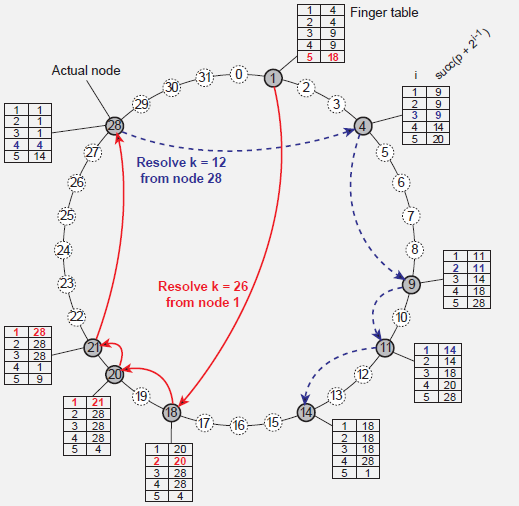
\includegraphics[width=0.6\linewidth]{img/dht}
    \caption{Példa DHT-re finger table-el.}
    \label{fig:dht}
\end{figure}

\subsubsection{Hierarchikus módszerek}

\noindent \textbf{Hierarchical Location Services(HLS)}: A hálózatot osszuk fel tartományokra, és mindegyik tartományhoz
tartozzon katalógus. Építsünk hierarchiát a katalógusokból.\\

\noindent A csúcsokban tárolt adatok:
\begin{itemize}
    \item	Az $E$ egyed címe egy levélben található.
    \item	A gyökértől az $E$ leveléig vezető úton minden belső csúcsban van egy mutató a lefelé következő csúcsra
          az úton.
    \item	Mivel a gyökér minden út kiindulópontja, minden egyedről van információja.
\end{itemize}

\noindent Keresés a fában: A kliens tartományából indul a keresés. Felmegyünk addig a fában, amíg olyan csúcshoz nem
érünk, amelyik tud $E$-ről, majd követjük a mutatókat a levélig, amely tudja $E$ címét. Mivel a gyökér minden
egyedet ismer, a terminálás garantált.\\

\noindent Beszúrás a fában: Ugyanaddig megyünk felfelé a fában, mint keresésnél, majd a belső csúcsokban mutatókat
helyezünk el.

\begin{figure}[H]
    \centering
    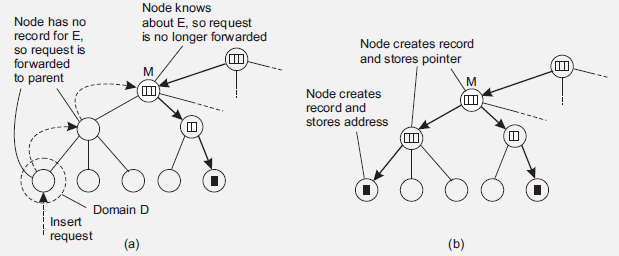
\includegraphics[width=0.8\linewidth]{img/hls_insert}
    \caption{Beszúrás a fában HLS-nél.}
    \label{fig:hls_insert}
\end{figure}

\subsection{Strukturált nevek}

\noindent \textbf{Névtér}: Gyökeres, irányított, élcímkézett gráf, a levelek tartalmazzák a megnevezett egyedeket,
a belső csúcsokat katalógusoknak vagy könyvtáraknak nevezzük. Az egyedhez vezető út címkéit összeolvasva
kapjuk az egyed egy nevét. A bejárt út, ha a gyökértől indul, abszolút útvonalnév, ha belső csúcsból indul,
relatív útvonalnév. Mivel egy egyedhez több út is vezethet, több neve is lehet.

\begin{figure}[H]
    \centering
    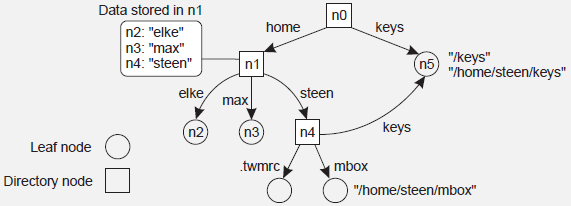
\includegraphics[width=0.8\linewidth]{img/nevter}
    \caption{Példa névtérre.}
    \label{fig:nevter}
\end{figure}

A névtér csúcsaiban (akár levélben, akár belső csúcsban) különféle attribútumokat is eltárolhatunk, pl. az egyed
típusát, azonosítóját, helyét/címét, más neveit, stb.\\

\noindent \textbf{Névfeloldás}: Kiinduló csúcsra van szükség a névfeloldás megkezdéséhez. A gyökér elérhetőségét
a név jellegétől függő környezet biztosítja, pl.:

\begin{itemize}
    \item	www.inf.elte.hu : egy DNS névszerver
    \item	/home/steen/mbox : a lokális NFS fájlszerver
    \item	0031204447784 : a telefonos hálózat
    \item	157.181.161.79 : a www.inf.elte.hu webszerverhez vezető út
\end{itemize}

\noindent \textbf{Névtér implementációja - DNS}: Ha nagy névterünk van, el kell osztani a gráfot a gépek között, hogy
hatékonnyá tegyük a névfeloldást és a névtér kezelését. Ilyen nagy névtér a DNS (Domain Name System).

\noindent A DNS névtérnek alapvetően 3 szintjét különböztetjük meg:

\begin{itemize}
    \item	Globális szint: Ide tartozik a gyökér és a felsőbb csúcsok (TLD-k, pl. országokhoz tartozó csúcsok - .hu, .uk, stb.).
          A szervezetek ezt közösen kezelik.

    \item	Szervezeti szint: Egy-egy szervezet által kezelt csúcsok szintje (pl. elte.hu, stb.).

    \item	Kezelői szint: Egy adott szervezeten belül kezelt csúcsok (pl. elte.hu-n belüli csúcsok)
\end{itemize}

\begin{figure}[H]
    \centering
    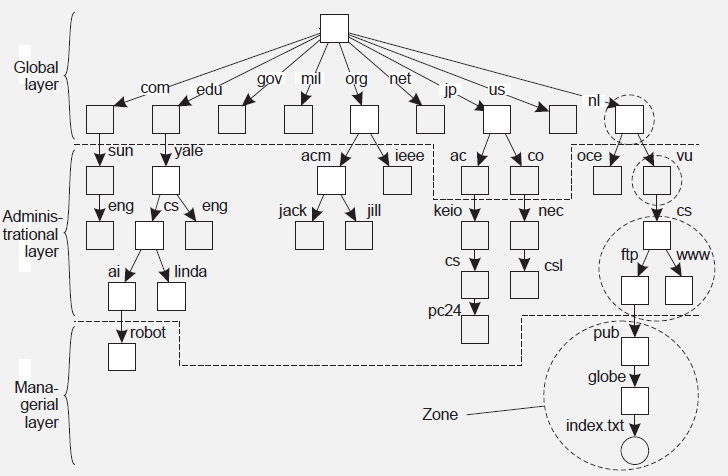
\includegraphics[width=0.8\linewidth]{img/dns}
    \caption{A DNS névtér egy része.}
    \label{fig:dns}
\end{figure}

\noindent \textbf{A névfeloldás különöző megközelítései}: DNS névtér esetén alapvetően két különböző névfeloldási
megközelítést alkalmazunk:

\begin{itemize}
    \item	Rekurzív névfeloldás: A rekurzív névfeloldás során a névszerverek egymás között kommunikálva oldják fel
          a neveket, a kliensoldali névfeloldóhoz rögtön a válasz érkezik.

    \item	Iteratív névfeloldás: A névfeloldást a gyökér névszerverek egyikétől indítjuk. Az iteratív névfeloldás
          során a névnek mindig csak egy komponensét oldjuk fel, a megszólított névszerver az ehhez tartozó névszerver
          címét adja vissza (ha a kliensoldali névfeloldó megkapja ezt a címet, a következő komponens feloldását ettől
          a névszervertől kéri - ez addig megy, míg teljesen fel nem oldjuk a nevet).
\end{itemize}

\noindent \textbf{Skálázhatóság}: Mivel sok kérést kell kezelni rövid idő alatt, ezért a globális szint névszerverei
nagy terhelést kapnának. Mivel a felső szinteken a gráf ritkán változik, ezért az ezeken a szinteken található
csúcsok adatairól több szerveren is tarthatunk másolatot, így a keresést közelebbről indíthatjuk (pl. van
több gyökér névszerver, a hozzánk legközelebbihez fordulunk).

\subsubsection{Attribútumalapú nevek}

Az egyedeket sokszor kényelmes lehet tulajdonságaik (attribútumaik) alapján keresni, viszont ha bármilyen
kombinációban megadhatunk attribútumértékeket, akkor a kereséshez az összes egyedet érintenünk kell, ami
nem hatékony. \\

\noindent \textbf{X.500, LDAP}: A katalógusszolgáltatásokban az attribútumokra megkötések érvényesek (X.500 szabvány), amelyet
az LDAP protokollon keresztül szokás elérni. Az elnevezési rendszer fastruktúrájú, élei attribútum-érték párokkal címzettek.
Az egyedekre az útjuk jellemzői vonatkoznak, és további párokat is tartalmazhatnak.

\section{Kommunikáció}

\subsection{Köztesréteg}

A köztesrétegbe (middleware) olyan szolgáltatásokat és protokollokat szokás sorolni, amelyek sokfajta
alkalmazáshoz lehetnek hasznosak és alapvetően a rendszer egyedei közötti összekötő kapocsként szolgálnak.

\begin{itemize}
    \item	Kommunikációs protokollok
    \item	Sorosítás (szerializáció, marshalling), adatok reprezentációjának átalakítása
    \item	Elnevezési protokollok az erőforrások megosztásának könnyítésére
    \item	Biztonsági protokollok a kommunikáció biztonságosabbá tételére
    \item	Skálázási mechanizmusok adatok replikációjára és gyorsítótárazására
\end{itemize}

\subsection{A kommunikáció fajtái}

A kommunikáció lehet:

\begin{itemize}
    \item	időleges (transient) vagy megtartó (persistent):
          \begin{itemize}
              \item	időleges: a kommunikációs rendszer elveti az üzenetet, ha az nem kézbesíthető
              \item	megtartó: a kommunikációs rendszer hajlandó huzamosabb ideig tárolni az üzenetet
          \end{itemize}
    \item	szinkron vagy aszinkron
          \begin{itemize}
              \item	szinkron: a küldő vár a válaszra, addig blokkolódik
              \item	aszinkron: a küldő nem vár a válaszra, hanem más tevékenységet folytat
          \end{itemize}
\end{itemize}

\subsubsection{Kliens-szerver modell}

A kliens-szerver modell jellemzően időleges, szinkron kommunikációt végez, ahol a kliensnek és a szervernek egyidejűleg
kell aktívnak lenni. A kliens a kérés küldése után blokkolódik, vár a szerver válaszára. A szerver csak a kliensek
fogadásával és a kérések feldolgozásával foglalkozik.

\subsubsection{Távoli eljáráshívás (RPC)}

A távoli eljáráshívásnál egy távoli gépen szeretnénk futtatni egy alprogramot. Ehhez hálózati kommunikáció szükséges,
amit elfedünk egy eljáráshívással.\\

\noindent \textbf{A hívás lépései}:

\begin{enumerate}
    \item	A kliensfolyamat lokálisan meghívja a klienscsonkot (client stub).
    \item	A klienscsonk becsomagolja az eljárás azonosítóját és paramétereit. Meghívja az oprendszert.
    \item	A lokális gép oprendszere elküldi a csomagot a távoli gép oprendszerének.
    \item	Az átadja az üzenetet a szervercsonknak (server stub).
    \item	A szervercsonk kicsomagolja az azonosítót és a paramétereket, amiket átad a szerverfolyamatnak.
    \item	A szerverfolyamat lokálisan meghívja az eljárást, megkapja a visszatérési értéket.
    \item	A visszatérési érték visszaküldése a kliensfolyamatnak hasonlóan történik, fordított irányban.
\end{enumerate}

\begin{figure}[H]
    \centering
    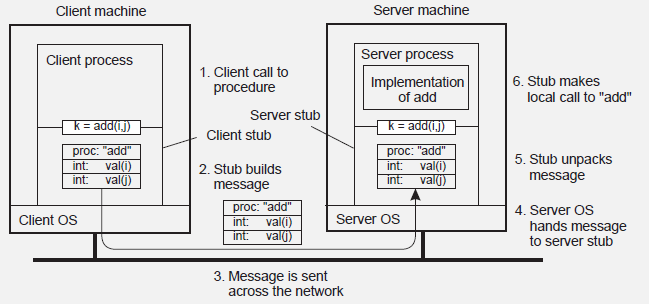
\includegraphics[width=0.8\linewidth]{img/rpc}
    \caption{A távoli eljáráshívás lépései.}
    \label{fig:rpc}
\end{figure}

\subsubsection{Socket}

Az időleges kommunikáció egy módja.

\begin{figure}[H]
    \centering
    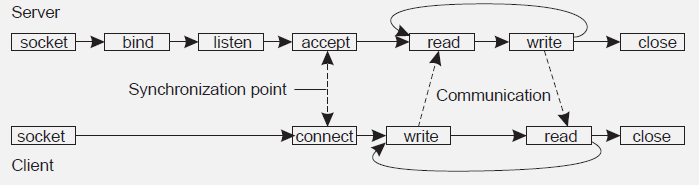
\includegraphics[width=0.8\linewidth]{img/socket}
    \caption{Kommunikáció socket-el.}
    \label{fig:socket}
\end{figure}

\subsubsection{Üzenetorientált köztesréteg (MOM)}

Az üzenetorientált köztesréteg (MOM - message-oriented middleware) egy megtartó, aszinkron kommunikációs architektúra.
Segítségével a folyamatok üzeneteket küldhetnek egymásnak. A küldő félnek nem kell a válaszra várnia, addig
foglalkozhat mással.

A MOM várakozási sorokat tart fenn a rendszer gépein. A kliensek az alábbi műveleteket
használhatják a várakozási sorokra:

\begin{itemize}
    \item	PUT: Üzenetet tesz a sor végére.
    \item	GET: Blokkol, amíg a sor üres, majd kiveszi az első üzenetet
    \item	POLL: Lekérdezi, hogy van-e üzenet. Ha van, leveszi az elsőt.
          Ha nincs, nem blokkol, folytatja a tevékenységét.
    \item	NOTIFY: Kezelőrutint telepít a várakozási sorhoz, amely minden
          beérkező üzenetre meghívódik.
\end{itemize}

Az üzenetsorkezelő rendszerek feltételezik, hogy a rendszer minden eleme közös protokollt használ, azaz az üzenetek
szerkezete és adatábrázolása megegyezik. A kérdés: mi van akkor, ha heterogén a rendszerünk? Erre szolgál
az üzenetközvetítő (message broker), amely heterogén rendszerben gondoskodik a megfelelő konverziókról, azaz
átalakítja az üzenetet a fogadó által használt formátumra. Általában proxy-ként is működik, azaz a közvetítés
mellett más funkciókat is nyújt, pl. biztonsági funkciókat.

\subsubsection{Folyam (stream)}

Az eddig tárgyalt kommunikációfajtákban közös, hogy az adategységek közötti időbeli kapcsolat nem befolyásolja
azok jelentését, folyamatos médiánál (pl. audio, videó, szenzoradatok) viszont az adatok időfüggőek, ezért a
kommunikáció időbeliségével kapcsolatban izokrón megkötést teszünk, ami felső és alsó korlátot is ad
a csomagok átvitelének idejére.\\

\noindent \textbf{Folyam}: Ilyen izokrón adatátvitelt lehetővé tevő kommunikációs forma a folyam. Főbb jellemzői:
\begin{itemize}
    \item	Egyirányú
    \item	Legtöbbször egy forrástól irányul egy vagy több nyelő felé
    \item	A forrás és/vagy nyelő gyakran közvetlenül kapcsolódik olyan hardverelemekhez, mint pl. egy kamera, képernyő,
          mikrofon, stb.
\end{itemize}

\noindent \textbf{Főbb típusai}:
\begin{itemize}
    \item	Egyszerű folyam: egyfajta adatot továbbít, pl. egyetlen audiocsatornát, vagy csak videót.
    \item	Összetett folyam: Többfajta adatot továbbít egyszerre, pl. videót többcsatornájú audióval (sztereó, 5.1, stb.).
          Az összetett folyam esetében biztosítani kell, hogy az alfolyamok a nyelőnél időben ne csússzanak el egymáshoz képest.
          Ennek egyik módja a szinkronizáció. Egy másik lehetséges módszer a multiplexálás és demultiplexálás. Ekkor a forrás
          egyetlen folyamot készít (multiplexálás). Itt az alfolyamok garantáltan szinkronban vannak egymással. A nyelőnél kell
          szétbontani a folyamot alfolyamokra (demultiplexálás).
\end{itemize}

\noindent \textbf{QoS}: A folyamokkal kapcsolatban sokfajta követelmény írható elő, ezeket összefoglaló néven
a szolgáltás minőségének (QoS - Quality of Service) nevezzük. Ilyen jellemzők például a következők:

\begin{itemize}
    \item	Az átviteli sebesség, azaz a bitráta.
    \item	A folyam elindításának legnagyobb megengedett késleltetése.
    \item	A folyam adategységeinek megadott idő alatt el kell jutniuk a forrástól a nyelőig.
    \item	Remegés (jitter): az adategységek beérkezési idejének egyenetlensége. Ennek csökkentésének
          egy módja a pufferelés.
\end{itemize}

\section{Szinkronizáció}

\subsection{Órák szinkronizálása}
Néha a pontos időt szeretnénk megtudni, néha elég, hogy ha két időpont közül megállapítható, hogy melyik volt korábban.
A világidő: UTC.\\

\subsubsection{Fizikai órák}

\noindent \textbf{A fizikai idő elterjesztése}: Ha a rendszerünkben van UTC-vevő, az megkapja a pontos időt. Ezt a
következők figyelembevételével terjeszthetjük el a rendszeren belül.

\begin{itemize}
    \item	A $p$ gép saját órája szerint az idő a $t$ UTC-időpillanatban $C_{p}(t)$
    \item	Ideális esetben az óra mindig pontos, azaz $C_{p}(t) = t$ minden $t$ UTC-időpillanatra. Másképpen
          fogalmazva az óra sebessége mindig 1, azaz $dC/dt = 1$.
    \item	A valóságban $p$ órája vagy túl gyors, vagy túl lassú, de viszonylag pontos:
          \begin{displaymath}
              1-\rho \leq \frac{dC}{dt} \leq 1+\rho
          \end{displaymath}

          \begin{figure}[H]
              \centering
              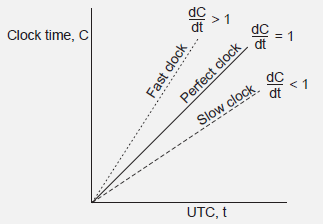
\includegraphics[width=0.4\linewidth]{img/clockspeed}
              \caption{Az óra sebessége.}
              \label{fig:clockspeed}
          \end{figure}
\end{itemize}

\noindent \textbf{Cristian algoritmusa}: Csak megadott $\delta$ eltérést akarunk megengedni az óra sebességében. Mindegyik
gép egy központi időszerverről kéri le a pontos időt legfeljebb $\frac{\delta}{2\rho}$ másodpercenként (ekkor tudunk $\delta$
eltérésen belül maradni). Az órát nem a megkapott időpontra kell állítani: bele kell számolni, hogy a szerver kezelte a kérést
és a válasznak vissza kellett érkeznie a hálózaton.\\

\noindent \textbf{Berkeley algoritmusa}: Nem a pontos idő beállítása a cél, csak az, hogy a rendszeren belül minden gép ideje
azonos legyen. Az időszerver időnként minden gép idejét bekéri, amiből átlagot von, majd mindenkit értesít, hogy a saját
óráját mennyivel kell átállítania. Az idő egyik gépnél sem folyhat visszafelé, ezért ha valamelyik órát vissza kellene állítani,
akkor ehelyett lelassítja az óráját addig, amíg a kívánt idő be nem áll.

\subsubsection{Logikai órák}

\noindent \textbf{Az előbb-történt reláció}: Az előbb-törént (happened-before) reláció az alábbi tulajdonságokkal bíró reláció.
Annak jelölése, hogy $a$ előbb történt, mint $b$: $a \to b$.

\begin{itemize}
    \item	Ha ugyanabban a folyamatban $a$ előbb következett be, mint $b$, akkor $a \to b$.
    \item	Ha $a$ esemény egy üzenet küldése, $b$ pedig ennek az üzenetnek a fogadása, akkor $a \to b$.
    \item	Tranzitív: Ha $a \to b$ és $b \to c$, akkor $a \to c$.
\end{itemize}

\noindent \textbf{Az idő és az előbb-történt reláció}: Minden $e$ eseményhez időbélyeget rendelünk, ami egy egész szám. Jelölése:
$C(e)$, és megköveteljük az alábbi tulajdonságokat:

\begin{itemize}
    \item	Ha $a \to b$ egy folyamat eseményeire, akkor $C(a)<C(b)$
    \item	Ha $a$ esemény egy üzenet küldése, $b$ pedig ennek az üzenetnek a fogadása, akkor $C(a)<C(b)$.
\end{itemize}

Ha van globális óra, akkor az időbélyeg elkészíthető. A továbbiakban azzal foglalkozunk, hogy mi van akkor, ha nincs globális
óra.\\

\noindent \textbf{Lampert-féle időbélyeg}: Minden $P_{i}$ folyamat egy $C_{i}$ számlálót tart nyilván az alábbiak szerint:
\begin{itemize}
    \item	$P_{i}$ minden eseménye eggyel növeli $C_{i}$-t.
    \item	Az elküldött $m$ üzenetre ráírjuk az időbélyeget: $ts(m) = C_{i}$.
    \item	Ha az $m$ üzenet beérkezik $P_{j}$ folyamathoz, ott a számláló új értéke
          $C_{j} = \max \left\{C_{j},ts(m)\right\}+1$ lesz
    \item	$P_{i}$ és $P_{j}$ egybeeső időbélyegjei közül tekintsük a $P_{i}$-belit elsőnek, ha $i<j$.
\end{itemize}

\noindent \textbf{Pontosan sorbarendezett csoportcímzés}: A $P_{i}$ folyamat minden műveletet időbélyeggel ellátott
üzenetben küld el. $P_{i}$ egyúttal beteszi a küldött üzenetet a saját $queue_{i}$ prioritásos sorába. A $P_{j}$
folyamat a beérkező üzeneteket az ő $queue_{j}$ prioritásos sorába teszi be az időbélyegnek megfelelő prioritással.
Az üzenet érkezéséről mindegyik folyamatot értesíti.
$P_{j}$ akkor adja át a $msg_{i}$ üzenet feldolgozásra, ha:
\begin{itemize}
    \item	$msg_{i}$ a $queue_{j}$ elején található, azaz az ő időbélyege a legkisebb
    \item	a $queue_{j}$ sorban minden $P_{k}, k \not = i$ folyamatnak megtalálható legalább egy üzenete, amelynek
          $msg_{i}$-nél későbbi az időbélyege

\end{itemize}

\noindent \textbf{Időbélyeg-vektor}:
\begin{itemize}
    \item	$P_{i}$ most már az összes folyamat idejét is számon tartja egy $VC_{i}[1..n]$ tömbben, ahol
          $VC_{i}[j]$ azon $P_{j}$-ben bekövetkezett események száma, amiről $P_{i}$ tud.

    \item	Az $m$ üzenet elküldése során $P_{i}$ megnöveli eggyel $VC_{i}[i]$ értékét és a teljes $VC_{i}$
          időbélyeg-vektort ráírja az üzenetre.

    \item	Amikor az $m$ üzenet megérkezik $P_{j}$-hez, amelyen a $ts(m)$ időbélyeg van, akkor
          \begin{enumerate}
              \item	$VC_{j}[k] := \max \left\{VC_{j}[k], ts_{m}[k]\right\}$
              \item	$VC_{j}[j]$ megnő eggyel
          \end{enumerate}
\end{itemize}

\subsection{Kölcsönös kizárás}

Több folyamat egyszerre szeretne hozzáférni egy adott erőforráshoz. Ezt egyszerre csak egynek engedhetjük meg
közülük, különben az erőforrás helytelen állapotba kerülhet.

\subsubsection{Kölcsönös kizárás központi szerver használatával}

Egy központi szerver a koordinátor, ő szabályozza az erőforráshoz való hozzáférést. Van egy várakozási sora.
Ha az erőforrás szabad, akkor ha kérés érkezik rá, a szerver megadja a hozzáférést és foglalttá teszi. Ezután
ha valaki más hozzá akar férni az erőforráshoz, akkor bekerül a várakozási sorba. Miután az első kliens
elengedte az erőforrást, az ahhoz kerül, aki a sor elején van. Ha kiürült a sor és az utolsó kliens is
elengedte az erőforrást, az újra szabaddá válik.

\begin{figure}[H]
    \centering
    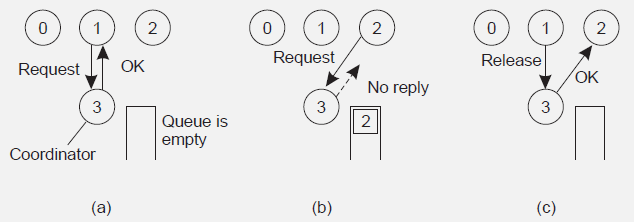
\includegraphics[width=0.6\linewidth]{img/kolcskizar_kozp}
    \caption{Példa központosított kölcsönös kizárásra.}
    \label{fig:kolcskizar_kozp}
\end{figure}

\subsubsection{Decentralizált kölcsönös kizárás}

Tegyük fel, hogy az erőforrás $n$-szeresen többszörözött, és minden replikátumhoz tartozik egy azt kezelő
koordinátor. A hozzáférésről többségi szavazás dönt: legalább $m$ koordinátor szükséges, ahol $m>\frac{n}{2}$.
Feltesszük, hogy egy esetleges összeomlás után a koordinátor felépül, de a kiadott engedélyeket
elfelejti.

\subsubsection{Elosztott kölcsönös kizárás}

Többszörözött az erőforrás. Amikor a kliens hozzá szeretne férni az erőforráshoz, kérést küld a koordinátornak
időbélyeggel ellátva. Választ (hozzáférési engedélyt) akkor kap, ha:

\begin{itemize}
    \item	A koordinátor nem igényli az erőforrást, vagy
    \item	a koordinátor is igényli az erőforrást, de kisebb az időbélyege.
    \item	Különben a koordinátor átmenetileg nem válaszol.
\end{itemize}

\begin{figure}[H]
    \centering
    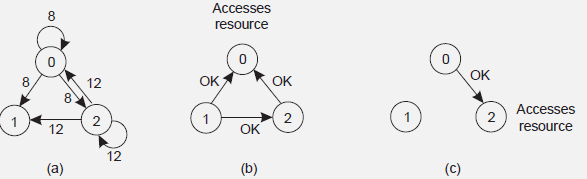
\includegraphics[width=0.6\linewidth]{img/kolcskizar_elosztott}
    \caption{Példa elosztott kölcsönös kizárásra.}
    \label{fig:kolcskizar_elosztott}
\end{figure}

\subsubsection{Kölcsönös kizárás token ring-gel}

A folyamatokat egy logikai gyűrűbe szervezzük. Egy tokent küldünk körbe. Amelyik folyamat birtokolja a tokent, az
férhet hozzá az erőforráshoz.

\subsection{Vezetőválasztás}

Sok algoritmusnak szüksége van arra, hogy kijelöljön egy folyamatot, amely a további lépéseket koordinálja.

\subsubsection{Zsarnok-algoritmus}

A folyamatoknak sorszámot adunk, melyek közül a legnagyobb sorszámút szeretnénk vezetőnek választani.\\

\noindent A zsarnok-algoritmus lépései:
\begin{enumerate}
    \item	A vezetőválasztás kezdeményezése. Bármelyik folyamat kezdeményezheti. Mindegyik olyan folyamatnak,
          amelyről nem tudja, hogy kisebb lenne az övénél a sorszáma, elküld egy üzenetet.

    \item	Ha a nagyobb sorszámú folyamat üzenetet kap egy kisebb sorszámútól, akkor visszaküld neki egy
          olyan üzenetet, amivel kiveszi a kisebb sorszámút a választásból.

    \item	Amelyik folyamat nem kap letiltó üzenet egy bizonyos időn belül, akkor ő lesz a vezető. Erről
          értesíti a többi folyamatot egy-egy üzenettel.
\end{enumerate}

\begin{figure}[H]
    \centering
    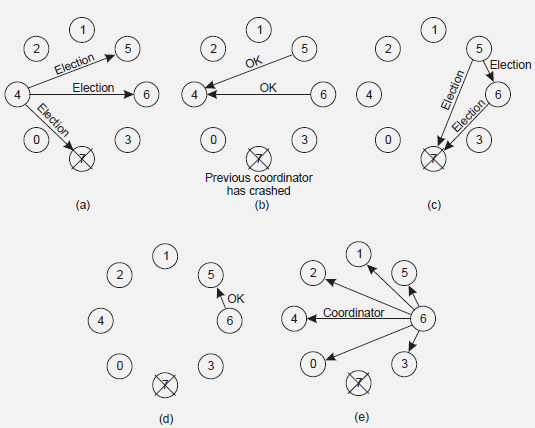
\includegraphics[width=0.6\linewidth]{img/zsarnok}
    \caption{Példa a zsarnok-algoritmus működésére.}
    \label{fig:zsarnok}
\end{figure}

\subsubsection{Vezetőválasztás gyűrűben}

Logikai gyűrűnk van, a folyamatoknak vannak sorszámai. A legnagyobb sorszámú folyamatot szeretnénk vezetőnek választani.
Bármelyik folyamat kezdeményezhet vezetőválasztást: elindít egy üzenetet a gyűrűn körbe, amelyre mindenki ráírja a
a sorszámát. Ha egy folyamat összeomlott, az kimarad az üzenetküldésből. Amikor az üzenet visszajut a kezdeményezőhöz,
minden aktív folyamat sorszáma szerepel rajta. Ezek közül a legnagyobb sorszámú lesz a vezető. Ezt egy másik
üzenet körbeküldése tudatja mindenkivel.

Ha több folyamat kezdeményez egyszerre választást, az nem probléma, ugyanaz az eredmény adódik. Ha az üzenetek
elvesznének, akkor újra lehet kezdeni a választást.

\subsubsection{Superpeer-választás}

A superpeer-eket úgy szeretnénk megválasztani, hogy teljesüljön rájuk:

\begin{itemize}
    \item	A többi csúcs alacsony késleltetéssel éri el őket.
    \item	Egyenletesen vannak elosztva a hálózaton.
    \item	A csúcsok megadott hányadát választjuk superpeer-nek.
    \item	Egy superpeer korlátozott számú peer-t szolgál ki.
\end{itemize}

\noindent \textbf{Megvalósítás DHT esetén}: Ha $m$-bites azonosítókat használunk, és $S$ superpeer-re van szükség, akkor
a $k= \lceil \log_{2} S \rceil$ felső bitet foglaljuk le a superpeer-ek számára. Így N csúcs esetén kb. $2^{k-m}N$
superpeer lesz.

A $p$ kulcshoz tartozó superpeer a $p$ AND $\underbrace{11...11}_{k}\underbrace{00..00}_{m-k}$ kulcs felelőse lesz.

\section{Konzisztencia}

\noindent \textbf{Konfliktusos műveletek}: A replikátumok konzisztensen tartásához biztosítani kell, hogy az egymással
konfliktusba kerülhető műveletek minden replikátumon egyforma sorrendben futnak le. Írás-olvasás és írás-írás
konfliktusok fordulhatnak elő.\\

\noindent \textbf{Konzisztenciamodell}: A konzisztenciamodell megszabja, milyen módokon használhatják a folyamatok
az adatbázist. Ha a feltételek teljesülnek, az adattárat érvényesnek tekintjük.\\

\noindent \textbf{Konzisztencia mértéke}: A konzisztencia többféle módon is sérülhet: eltérhet a replikátumok
számértéke, frissessége, meg nem történt frissítési műveletek száma.\\

\noindent \textbf{Conit}: Az olyan adategység, amelyre közös feltételrendszer vonatkozik, a conit (consistency unit).

\subsection{Soros konzisztencia}

A feltételeket nem számértékekre, hanem írások/olvasások tényére alapozzuk.
Jelölések:
\begin{itemize}
    \item	W(x) : x változót írta a folyamat
    \item	R(x) : x változót olvasta a folyamat
\end{itemize}

Soros konzisztencia esetén azt várjuk el, hogy a végrehajtás eredménye olyan legyen, mintha az összes folyamat
összes művelete egy meghatározott sorrendben történt volna meg, megőrizve bármely adott folyamat saját műveletinek
sorrendjét.

\begin{figure}[H]
    \centering
    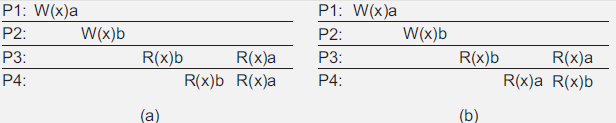
\includegraphics[width=0.7\linewidth]{img/konz_soros}
    \caption{Példa: az (a) teljesíti, (b) nem a soros konzisztencia követelményeit.}
    \label{fig:konz_soros}
\end{figure}

\subsection{Okozati konzisztencia}

A potenciálisan okozati összefüggésben álló műveleteket kell mindegyik folyamatnak azonos sorrendben látnia.
A konkurens írásokat a különböző folyamatok különböző sorrendben láthatják.

\begin{figure}[H]
    \centering
    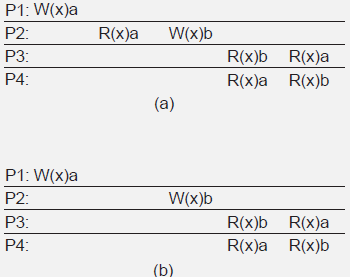
\includegraphics[width=0.4\linewidth]{img/konz_okozati}
    \caption{Példa: a (b) teljesíti, (a) nem az okozati konzisztencia követelményeit.}
    \label{fig:konz_okozati}
\end{figure}

\subsection{Kliensközpontú konzisztencia}

Azt helyezzük most előtérbe, hogy a szervereken tárolt adatok hogyan látszanak egy adott kliens számára. A kliens
mozog: különböző szerverekhez csatlakozik, és írási/olvasási műveleteket hajt végre.

Az $A$ szerver után a $B$ szerverhez csatlakozva különböző problémák léphetnek fel:

\begin{itemize}
    \item	Az $A$-ra feltöltött frissítések lehet, hogy nem jutottak még el $B$-hez.
    \item	$B$-n lehet, hogy újabb adatok találhatóak, mint $A$-n.
    \item	A $B$-re feltöltött frissítések ütközhetnek az $A$-ra feltöltöttekkel.
\end{itemize}

A cél az, hogy a kliens azokat az adatokat, amiket az $A$ szerveren kezelt, ugyanolyan állapotban
lássa $B$-n is. Ekkor az adatbázis konzisztensnek látszik a kliens számára.\\

\subsubsection{Monoton olvasás}
Ha egyszer a kliens kiolvasott egy értéket $x$-ből, minden ezután következő
olvasás ezt adja, vagy ennél frissebb értéket.

Például levelezőkliens esetén minden korábban letöltött levelünknek meg kell lennie az új szerveren is.

\subsubsection{Monoton írás}

A kliens akkor írhatja $x$-et, ha kliens korábbi írásai $x$-re már befejeződtek.

Például verziókezelésnél minden korábbi verziónak meg kell lennie a szerveren, ha új verziót akarunk feltölteni.

\subsubsection{Olvasd az írásodat}

Ha kliens olvassa $x$-et, a saját legutolsó írásának eredményét kapja, vagy frissebbet.

Például a kliens a honlapját szerkeszti, majd megnézi az eredményt. Ahelyett, hogy a böngésző gyorsítótárából
egy régebbi változat kerülne elő, a legfrissebbet szeretné látni.

\subsubsection{Írás olvasás után}

Ha a kliens kiolvasott egy értéket $x$-ből, minden ezután kiadott frissítési művelete $x$-nek legalább
ennyire friss értékét módosítja.

Például egy fórumon a kliens csak olyan hozzászólásra tud válaszolni, amit már látott.

\subsection{Tartalom replikálása}

Különböző jellegű folyamatok tárolhatják a másolatokat:

\begin{itemize}
    \item	Tartós másolat: eredetszerver (origin server)
    \item	Szerver által kezdeményezett másolat: replikátum kihelyezése egy szerverre, amikor az igényli
          az adatot
    \item	Kliens által kezdeményezett másolat: kliensoldali gyorsítótár
\end{itemize}

\subsubsection{Frissítés terjesztése}
Megváltozott tartalmat több különféle módon lehet kliens-szerver architektúrában átadni:

\begin{itemize}
    \item	Kizárólag  a frissítésről szóló értesítés/érvénytelenítés elterjesztése.
    \item	Passzív replikáció: adatok átvitele egyik másolatról a másikra
    \item	Aktív replikáció: frissítési művelet átvitele
\end{itemize}

A frissítést kezdeményezheti a szerver (küldésalapú frissítés), ekkor a szerver a kliens kérése nélkül elküldi a frissítést
a kliensnek, vagy kezdeményezheti a kliens, aki kérvényezi a frissítést a szervertől (rendelésalapú frissítés).\\

\noindent \textbf{Haszonbérlet (lease)}: A szerver ígéretet tesz a kliensnek, hogy átküldi a frissítést, amíg a haszonbérlet aktív.

\end{document}